%%%%%%%%%%%%%%%%%%%%%%%%%%%%%%%%%%%%%%%%%%%%%%%%%%%%%%%%%%%%%%%%%%%%%%
%%%%%%%%%%%%%%%%%%%%%%%%%%%%%%%%%%%%%%%%%%%%%%%%%%%%%%%%%%%%%%%%%%%%%%
\documentclass[dvips,portrait]{seminar}             %%%%%%%%%%%%%%%%%%
                                                    %%%%%%%%%%%%%%%%%%
%%%%%%%%%%%%%%%%%%%%%%%%%%%%%%%%%%%%%%%%%%%%%%%%%%%%
% gmake afb_sig-ps
%======================
%\def\Energy{MZ-1.8GeV (had.)}
\input Energy.tex
\input Process.tex
\def\Angle{$\theta^{\bullet}$}

%%%%%%%%%%%%%%%%%%%%%%%%%%%%%%%%%%%%%%%%%%%%%%%%%%%%%%%
%%%%%%%%%%%%%%%%%%%%%%%%%%%%%%%%%%%%%%%%%%%%%%%%%%%%%%%
\begin{document}                     %%%%%%%%%%%%%%%%%%


%//////////////////////////////////////////////////////////////////////////////////
%//////////////////////////////////////////////////////////////////////////////////
%//////////////////////////////////////////////////////////////////////////////////
\begin{slide}
\titbox{{\bf\Color{Red} CEEX $\sigma$ and $A_{\rm FB}$, energy cut-off study }}

\vspace{-1mm}
\setlength{\unitlength}{1mm}
{\small\Color{Blue}
%  $e^-e^+ \to f\bar{f}$, $f=\mu^-$, at \Energy.
  \Process, at \Energy.
  Energy cut: $v<v_{\max}$, $v=1-M^2_{f\bar{f}}/s$.\\
  Scattering angle for $A_{\rm FB}$ is $\theta=$\Angle.
  No cut in \Angle.
  E-W corr. in \KK\  according to DIZET 6.x.\\
  EEX3 is \OrderLL{\alpha^3} EEX3 matrix element without ISR$\otimes$FSR interf.\\
  \KK{}sem is semianalytical part of \KK.
  {\tiny (Angle $\theta^{\bullet}$ is from Phys. Rev. {\bf D41}, 1425 (1990).)}
}
\vspace{-1mm}
\begin{center}
\begin{picture}(95,54)
\put(-2, 00){\makebox(0,0)[lb]{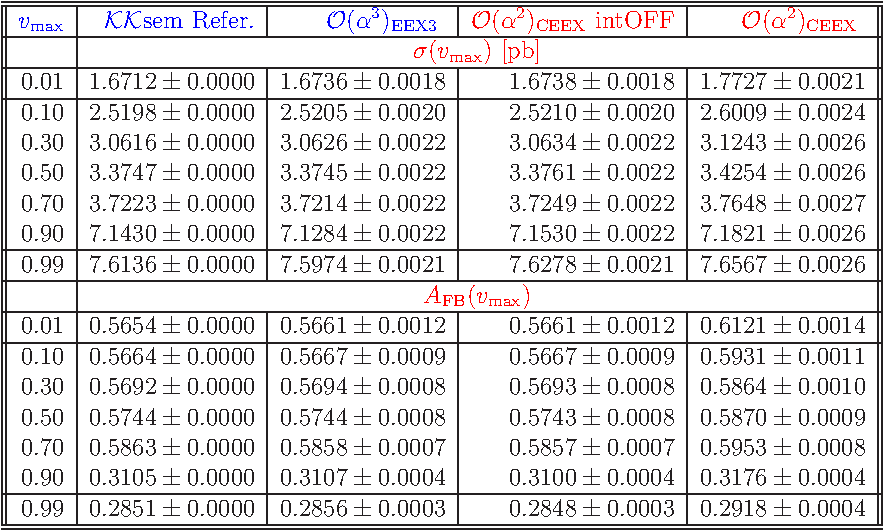
\epsfig{file=afb_int2-tab1.eps,width=95mm,height=54mm}}}
\end{picture}
\end{center}
%-----------------------------------------------------------
\vfill
\end{slide}   %%%
%%%%%%%%%%%%%%%%%%


%//////////////////////////////////////////////////////////////////////////////////
%//////////////////////////////////////////////////////////////////////////////////
%//////////////////////////////////////////////////////////////////////////////////
\begin{slide}
\titbox{{\large\bf\Color{Magenta} Total cross section $\sigma$, energy cut-off stydy}}

{\small\Color{Blue}
  The same as in the table. No cut in \Angle.
  Ref. $\sigma_{\rm ref}$ = semianalytical of \KK{}sem.
}
\begin{center}
\setlength{\unitlength}{1mm}
\begin{picture}(75,60)
%#####\put(0,0){\framebox( 70,60){ }}
\put(-2, 00){\makebox(0,0)[lb]{
\epsfig{file=afb_int2-Gsig.eps,width=75mm,height=60mm}
}}
\end{picture}
\end{center}
%-----------------------------------------------------------
\vfill
\end{slide}   %%%
%%%%%%%%%%%%%%%%%%

%//////////////////////////////////////////////////////////////////////////////////
%//////////////////////////////////////////////////////////////////////////////////
%//////////////////////////////////////////////////////////////////////////////////
\begin{slide}
\titbox{{\large\bf\Color{Magenta} Charge asymmetry $A_{\rm FB}$, energy cut-off study}}

{\small\Color{Blue}
  The same as in the table.
  No cut in \Angle.
  Reference $A_{\rm FB}^{\rm ref}$ =  semianalytical \KK{}sem.
}

\begin{center}
\setlength{\unitlength}{1mm}
\begin{picture}(75,60)
%#####\put(0,0){\framebox( 75,60){ }}
\put(-2, 00){\makebox(0,0)[lb]{
\epsfig{file=afb_int2-Gafb.eps,width=75mm,height=60mm}
}}
\end{picture}
\end{center}
%-----------------------------------------------------------
\vfill
\end{slide}   %%%
%%%%%%%%%%%%%%%%%%

%//////////////////////////////////////////////////////////////////////////////////
%//////////////////////////////////////////////////////////////////////////////////
%//////////////////////////////////////////////////////////////////////////////////
\begin{slide}
\titbox{{\large\bf\Color{Magenta} 
                      Physical Precision of CEEX ISR }}

{\small\Color{Blue}
  The difference between second and first order CEEX results for at \Energy.\\
  The energy cut is on $s'/s$, where $s'=m^2_{f\bar{f}}$.}\\
{\small\Color{Blue} Scattering angle is $\theta=$\Angle. }\\
{\tiny\Color{Blue}  [Angle $\theta^{\bullet}$ is defined in Phys. Rev. {\bf D41}, 1425 (1990)]}

%-----------------------------------------------------------
\begin{center}
\setlength{\unitlength}{1mm}
%
\begin{picture}(50,45)
\put(-1, 0){\makebox(0,0)[lb]{
\epsfig{file=afb_int2-sigHO.eps,width=50mm,height=45mm}
}}\end{picture}
%
\begin{picture}(45,45)
\put(-1, 0){\makebox(0,0)[lb]{
\epsfig{file=afb_int2-afbHO.eps,width=50mm,height=45mm}
}}\end{picture}
\vfill
\end{center}
%-----------------------------------------------------------
\vfill
\end{slide}   %%%
%%%%%%%%%%%%%%%%%%




\end{document}

